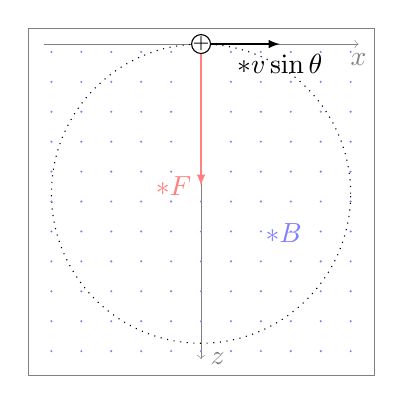
\begin{tikzpicture}[scale=1]
    \draw[gray,ultra thin] (-2.2,+0.2) rectangle (2.2,-4.2);
    \draw[->,gray,very thin] (-2,0)--(+2,0) node [below] {$x$};
    \draw[->,gray,very thin] (0,0)--(0,-4) node [right] {$z$};
    \draw[dotted] (0,-1.9) circle (1.9);
    
    \foreach \x in {-1.9,-1.52,...,1.9}
    {
        \foreach \y in {-0.1,-0.48,...,-3.9}
        {
            \fill[blue!50!white] (\x,\y) circle (0.015);
        }
    }

    \draw[-latex] (0,0)--(1,0) node [below] {$\vb*{v}\sin\theta$};
    \draw[-latex,red!50!white] (0,0)--(0,-1.8) node [left] {$\vb*{F}$};

    \draw[fill=white] (0,0,0) circle (0.12) node {\scriptsize $+$};

    \node[blue!50!white] at (1.05,-2.4) {$\vb*{B}$};
\end{tikzpicture}
